\textit{This page contains some how-to descriptions which should be deleted when the first draft of this thesis document is delivered by the M2GoParticipant.}

\textit{Figure \ref{fig:m2go_parts} shows an overview of the different M2Go parts. For each part, an own chapter exists. For each exercise a section should be created. The different tasks of the exercise are structured in subsections.}

%
\begin{figure}[H]
	\centering
	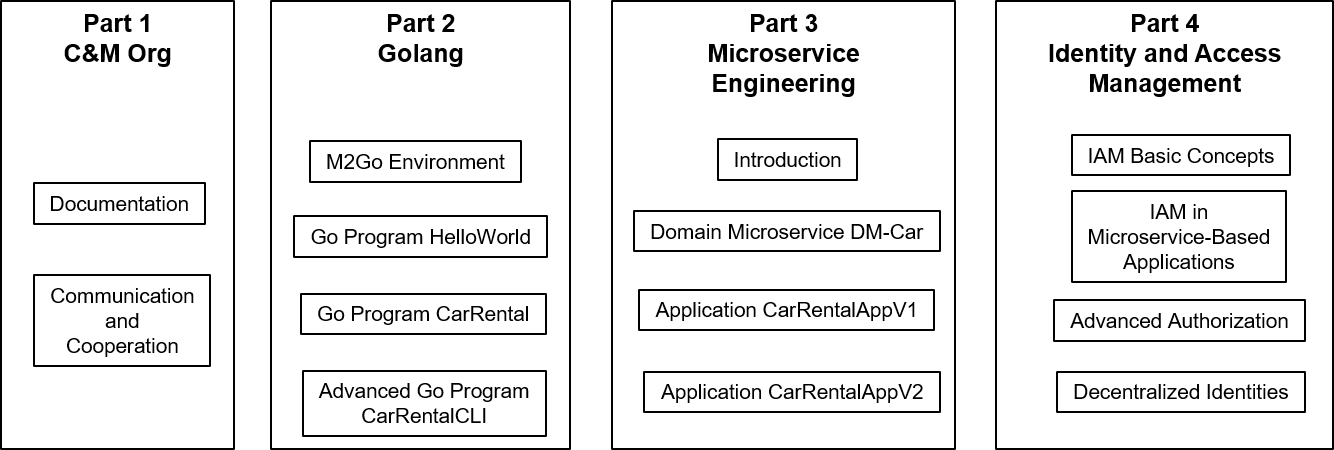
\includegraphics[width=0.8\textwidth]{figures/m2go_parts.png}
	\caption{M2Go Parts}
	\label{fig:m2go_parts}
\end{figure}
%


\textit{A code artifact is included in the thesis as follows (see Listing \ref{lst:code_artifact}).}

\begin{lstlisting}[caption = {Example for Code Artifacts in the Thesis}, label = {lst:code_artifact}, style = kit-cm]
First line of code artifact
Second line of code artifact
...
\end{lstlisting}

\textit{For writing and formatting rules, see \cite{CM-T-CMW}.}